% file: sections/appendix.tex

\section{附录}

\appendix

% file: sections/bib.tex

%%%%%%%%%%%%%%%%%%%%
\begin{frame}[allowframebreaks]
  \printbibliography
\end{frame}
%%%%%%%%%%%%%%%%%%%%


%%%%%%%%%%%%%%%%%%%% Begin: Jupiter %%%%%%%%%%%%%%%%%%%%

%%%%%%%%%%%%%%%%%%%%
\begin{frame}{}
  \begin{cdef}[最终收敛性 (Eventual Convergence)~\ncite{Ellis:SIGMOD89}]
    当用户不再提交更新操作时, 所有 replicas 上的列表是相同的。
  \end{cdef}

  \pause
  \vspace{0.50cm}

  \begin{cdef}[强最终一致性 (Strong Eventual Consistency)~\ncite{Shapiro:SSS11}]
    如果两个 replicas 处理了同一组更新操作, 则它们的列表是相同的。
  \end{cdef}

  \pause
  \vspace{0.60cm}
  \centerline{\red{\large 对系统的\red{中间状态}缺少足够的约束}}
\end{frame}
%%%%%%%%%%%%%%%%%%%%

%%%%%%%%%%%%%%%%%%%%
\begin{frame}{}
  \centerline{\large 针对列表的操作转换函数~\ncite{Ellis:SIGMOD89}}

  \resizebox{\textwidth}{!}{
    \begin{minipage}{\textwidth}
      % file: parts/list-ot.tex

\newcommand{\ldel}{\textsc{Del}}	% List DEL
\newcommand{\lins}{\textsc{Ins}}	% List INS
\newcommand{\ldelop}[2]{\ldel\left(#1, #2\right)}  % #1: index, #2: priority
\newcommand{\linsop}[3]{\lins\left(#1, #2, #3\right)}  % #1: index, #2: element, #3: priority

%%%%%%%%%% list-ot.tex %%%%%%%%%% 
\begin{align*}
  % ins vs. ins
  OT\Big(\lins(a_1, p_1, pr_1), \lins(a_2, p_2, pr_2)\Big) &= \begin{cases}
    \lins(a_1, p_1, pr_1) 		& p_1 < p_2 \\[3pt]
    \lins(a_1, p_1 + 1, pr_1) 		& p_1 > p_2 \\[3pt]
    \textsc{NOP} 			& p_1 = p_2 \land a_1 = a_2 \\[3pt]
    \lins(a_1, p_1 + 1, pr_1) 		& p_1 = p_2 \land a_1 \neq a_2 \land pr_1 > pr_2 \\[3pt]
    \lins(a_1, p_1, pr_1)		& p_1 = p_2 \land a_1 \neq a_2 \land pr_1 \le pr_2
  \end{cases} \\[10pt]
  % ins vs. del
  OT\Big(\lins(a_1, p_1, pr_1), \ldel(\_, p_2, pr_2)\Big) &= \begin{cases}
    \lins(a_1, p_1, pr_1) 		& p_1 \le p_2 \\[3pt]
    \lins(a_1, p_1 - 1, pr_1) 		& p_1 > p_2
  \end{cases} \\[10pt]
  % del vs. ins
  OT\Big(\ldel(\_, p_1, pr_1), \lins(a_2, p_2, pr_2)\Big) &= \begin{cases}
    \ldel(\_, p_1, pr_1) 		& p_1 < p_2 \\[3pt]
    \ldel(\_, p_1 + 1, pr_1) 		& p_1 \ge p_2
  \end{cases} \\[10pt]
  % del vs. del
  OT\Big(\ldel(\_, p_1, pr_1), \ldel(\_, p_2, pr_2)\Big) &= \begin{cases}
    \ldel(\_, p_1, pr_1) 		& p_1 < p_2 \\[3pt]
    \ldel(\_, p_1 - 1, pr_1) 		& p_1 > p_2 \\[3pt]
    \textsc{NOP}			& p_1 = p_2
  \end{cases} \\
\end{align*}
%%%%%%%%%% list-ot.tex %%%%%%%%%% 

    \end{minipage}
  }
\end{frame}
%%%%%%%%%%%%%%%%%%%%
%%%%%%%%%%%%%%%%%%%% End: Jupiter %%%%%%%%%%%%%%%%%%%%

%%%%%%%%%%%%%%%%%%%% Begin: VPC %%%%%%%%%%%%%%%%%%%%

%%%%%%%%%%%%%%%
\begin{frame}{}
  \begin{ctheorem}[\rwclosure{} 算法正确性]
    \begin{center}
      \emph{\vpc{mu}} 实例满足 \emph{\PRAM{}} 一致性 \\[5pt]
      $\iff$ \\[5pt]
      \rwclosure{} 算法所得图是 \emph{DAG} 图
    \end{center}
  \end{ctheorem}

  \pause
  \vspace{0.20cm}

  \begin{cproof}
    \begin{description}
      \item[``$\Longrightarrow$''] 反证法
      \item[``$\Longleftarrow$''] 
	\textcolor{red}{难点:} DAG 图蕴含着多个全序

	\textcolor{red}{技巧:} 对读操作作数学归纳, 构造合法调度
    \end{description}
  \end{cproof}

  \pause
  \vspace{0.30cm}

  \rwclosure{} 算法复杂度: 
  \[
    \underbrace{O(n^2)}_{\textrm{\#loops}} \quad\cdot
	\underbrace{O(n^3)}_{\textrm{transitive closure}}  = O(n^5)
  \]
\end{frame}
%%%%%%%%%%%%%%%

%%%%%%%%%%%%%%%
\begin{frame}{}
  \readcentric{} 算法复杂度: 
  \[
    \underbrace{O(n)}_{\textrm{iterations}} \cdot
	\underbrace{O(n \cdot n^2)}_{\textcolor{red}{\textsc{Topo-Schedule}}} = O(n^4)
  \]

  \vspace{0.30cm}
  \begin{clemma}[\textsc{Topo-Schedule} 的非迭代性]
    \begin{center}
      设\textsc{Topo-Schedule} 正在处理读操作$r$,\\
      则\textcolor{blue}{局部子图}中的每个写操作\textcolor{red}{最多只有一次机会}\\
      在满足规则 $w'wr$ 的三元组中扮演``$w'$角色''。
    \end{center}
  \end{clemma}
\end{frame}
%%%%%%%%%%%%%%%

%%%%%%%%%%%%%%%
\begin{frame}{实验评估}
  实验目的~\footnotemark[1]~\footnotetext[1]{机器配置: Intel Core i7 3.40GHZ, 4GB RAM.}:
  \begin{enumerate}
    \item 考察 \readcentric{} 算法的实际效率 
      \textcolor{blue}{\small ({\it vs.} 渐近时间复杂度)}
    \item 对比 \readcentric{} 算法与 \rwclosure{} 算法的效率
  \end{enumerate}

  \pause
  \vspace{0.50cm}

  两类负载:
  \begin{enumerate}
    \item 随机生成的系统执行
    \item 满足 \PRAM{} 一致性的系统执行 \textcolor{red}{\small ($\approx$ 最坏情况输入)}
  \end{enumerate}
\end{frame}
%%%%%%%%%%%%%%%

%%%%%%%%%%%%%%%
\begin{frame}{}
  \begin{figure}[t]
    \centering
    \begin{subfigure}[t]{0.50\textwidth}
      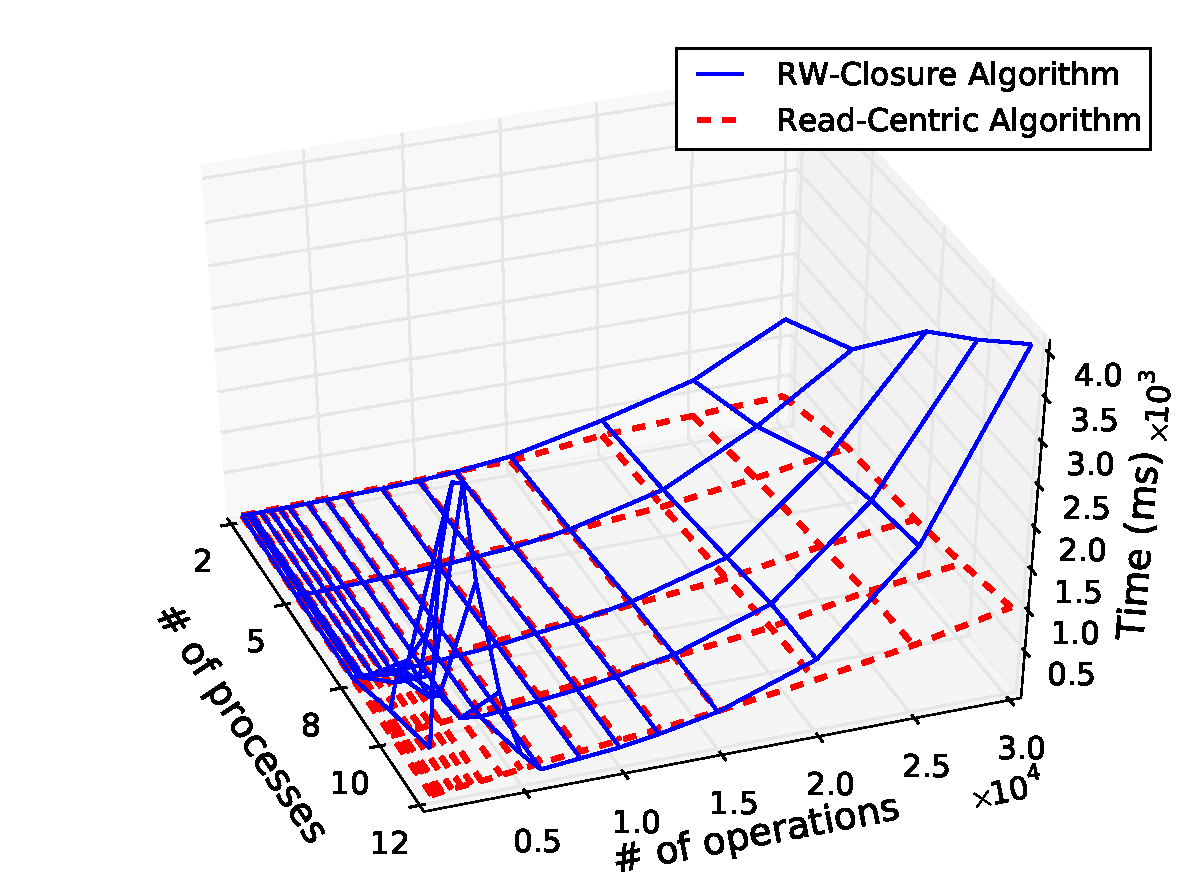
\includegraphics[width = 0.80\textwidth]{figs/vpc-random-cmp.pdf}
    \end{subfigure}%
    ~
    \begin{subfigure}[t]{0.50\textwidth}
      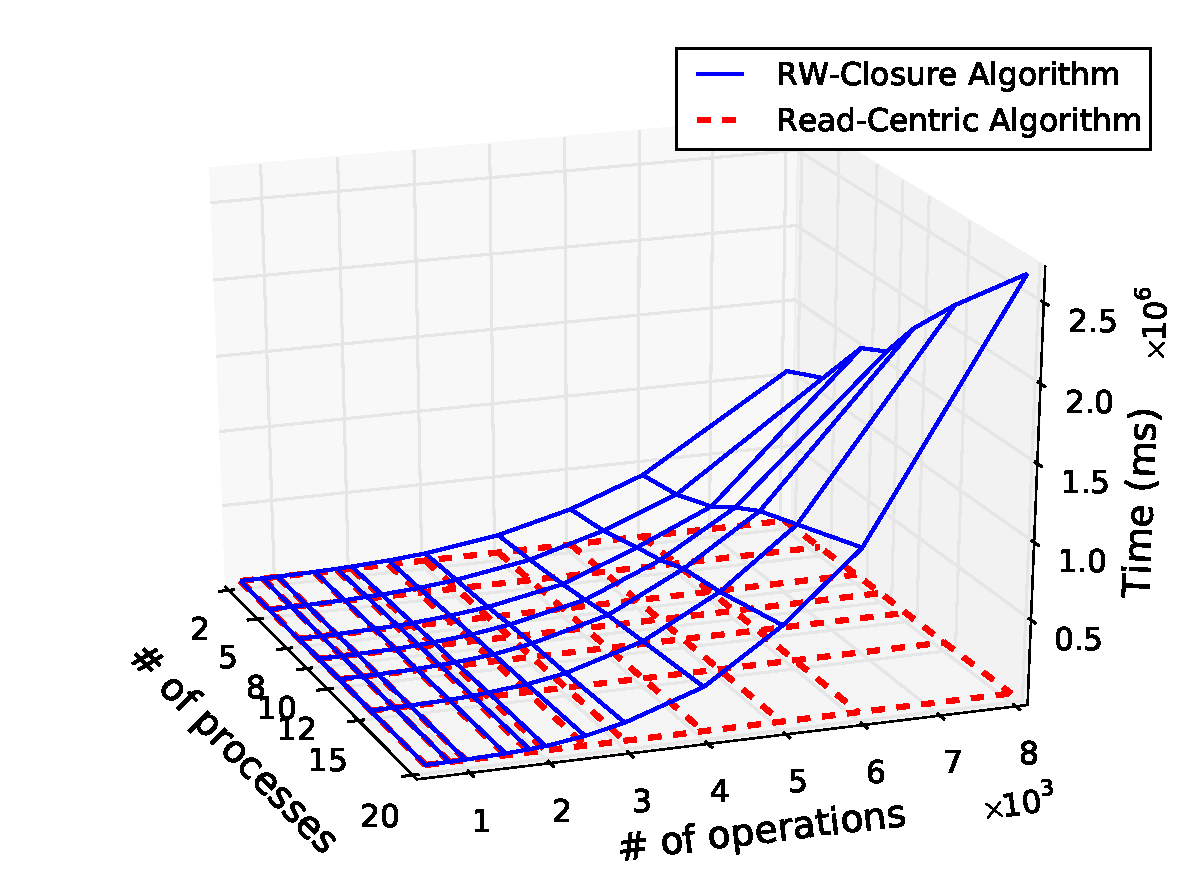
\includegraphics[width = 0.80\textwidth]{figs/vpc-valid-cmp.pdf}
    \end{subfigure}
    \caption{\rwclosure{} 算法与 \readcentric{} 算法在
    \textcolor{blue!80}{ (左) 随机生成}的执行及
    \textcolor{red!80}{ (右) 满足 \PRAM{} 一致性}的执行上的运行时间。}
  \end{figure}

  \pause
  \begin{center}
    \textcolor{red}{(右)} 20个进程、8,000 个操作: 

    \readcentric{} 可获得 694 倍加速.
  \end{center}
\end{frame}
%%%%%%%%%%%%%%%

%%%%%%%%%%%%%%%
\begin{frame}{}
  \fig{width = 0.45\textwidth}{figs/vpc-scalability-more.pdf}
  {\readcentric{} 算法在满足 \PRAM{} 一致性的执行上的运行时间}

  \vspace{-0.30cm}

  \begin{description}
    \centering
    \item[\readcentric{}:] 20个进程、60,000个操作 < 600s~\footnotemark[1]~\footnotetext[1]{用于测试, 规模可用}
    \item[\rwclosure{}:] 20个进程、8,000个操作 > 3,000s
  \end{description}
\end{frame}
%%%%%%%%%%%%%%%

%%%%%%%%%%%%%%%
\begin{frame}{}
  \begin{center}
    \hl{\large $\mathcal{I}$-Atomicity = $i$-实时序 + 读写语义}
  \end{center}

  \vspace{0.60cm}
  \centerline{$\mathcal{I}$: Inversions}

  \pause
  \vspace{0.30cm}
  \[
    f(\set{\text{inversions}}) \le i
  \]

  \pause
  \vspace{0.50cm}
  \centerline{\large 定义\red{框架}}
\end{frame}
%%%%%%%%%%%%%%%
%%%%%%%%%%%%%%%%%%%% End: VPC %%%%%%%%%%%%%%%%%%%%

%%%%%%%%%%%%%%%%%%%% Begin: Future Work %%%%%%%%%%%%%%%%%%%%
%%%%%%%%%%%%%%%
\begin{frame}{}
  \begin{center}
    ($50$种) \hl{一致性模型}关系图 \ncite{Viotti:CSUR16} \ncite{Burckhardt:Book14}
  \end{center}

  \fignocaption{width = 0.95\textwidth}{figs/non-transactional-consistency-models}

  \centerline{\red{\large 建立统一的形式化框架}}
\end{frame}
%%%%%%%%%%%%%%%%%%%% End: Future Work %%%%%%%%%%%%%%%%%%%%
